\subsection{GameController}
GameController klassen, holder styr på hele spillet. GameController har en konstruktør som tager imod parameter af typen Translator, det gør det muligt at oversætte alle tekststrenge i spillet. I konstruktøren bliver alle de forskellige klasser oprettet og gemt i lokale variabler.

\begin{figure}[H]
    \centering
    \includegraphics[width=\textwidth]{sources/7_implementering/gameKonstruktør.PNG}
    \caption{Konstruktør i GameController}
    \label{fig:KSGC}
\end{figure}

Klassen har en GameSetup metode som starter spilleren op med navn, farve og brik. Play metoden, er her hvor spillet bliver spillet. Det er her hvor spillerene kaster terninger, køber huse og udføre handlinger alt efter hvilket felt de er landet på. 

\begin{figure}[H]
    \centering
    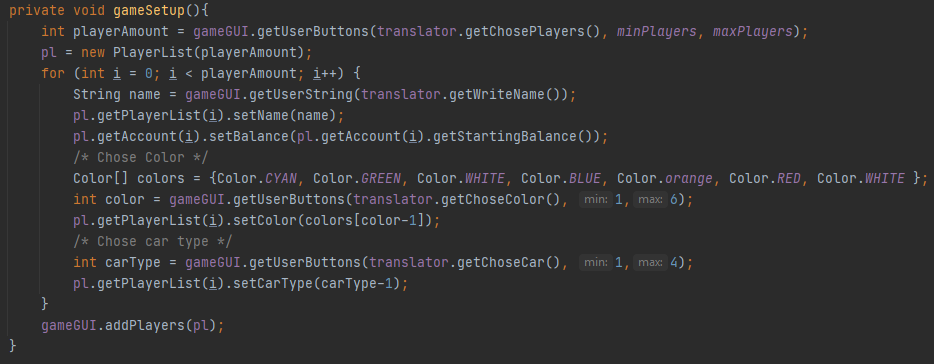
\includegraphics[width=\textwidth]{sources/7_implementering/gamesetup.PNG}
    \caption{GameSetup metoden i GameController}
    \label{fig:GS}
\end{figure}

Mange af de andre controller og klasser, bliver oprettet og taget i brug i denne klasse. Klasserne bliver brugt i GameController til at udføre handlinger på andre felter osv.